\documentclass{article}
\usepackage{tikz}
\usetikzlibrary{shapes.geometric, arrows, positioning, calc}

\begin{document}

\begin{tikzpicture}
  % Node definitions
  \node[circle,draw] (a) {*};
  \node[square, draw, right=of a] (b) {2};
  \node[circle, fill=blue!30, below=of a] (c) {3};
  \node[circle, draw, fill=red!20] (d) at (5, 5) {f};
  \node[circle, fill=black, label=below:A, draw] (e) at (6, 6) {};
  \node[circle, draw] (f) at (8, 8) {1};

  % Connections
  \draw[->] (a) -- node[above] {1} (b);
  \draw[->] (a) -- node[right] {2} (c);
  \draw[->] (b) -- node[right] {3} (c);
  \draw[->, bend right] (e) to (f);
\end{tikzpicture}


%\begin{tikzpicture}
%%nodes
%\node[circle,draw] (a) {A};
%\node[circle,draw,above=of a] (b) {B};
%\node[circle,draw,right=of a] (c) {C};
%\node[circle,draw,above=of c] (d) {D};
%\node[circle,draw,right=of c] (e) {E};
%
%%connections
%\draw[->](a)--(b);
%\draw[->](a)--(c);
%\draw[->](e)--(c);
%\draw[->](c)--(d);
%\draw[->](a)--(d);
%\draw[->](d)--(b);
%\draw[->, bend left=30](d) to (e);
%\draw[->, bend left=30] (e) to (d);
%\end{tikzpicture}

%\begin{tikzpicture}
%\node[circle, draw, fill=red!20] (a) at (0, 0) {F};
%\node[circle, draw, fill=blue!20] (b) at (4, 0) {C};
%\node[circle, draw, fill=pink!20] (c) at (1, -2) {E};
%\node[circle, draw, fill=yellow!20] (d) at (3, -2) {D};
%\node[circle, draw, fill=orange!20] (e) at (1, 2) {A};
%\node[circle, draw, fill=red!40] (f) at (3, 2) {B};
%
%%connections
%\draw[->,loop above] (a)to(a);
%\draw[->,loop above] (d)to(d);
%\draw[->] (a)to(e);
%\draw[->] (a)to(c);
%\draw[->] (d)to(b);
%\draw[->,bend left=30](c)to(d);
%\draw[->,bend left=30](d)to(c);
%\draw[->,bend left=30](b)to(f);
%\draw[->,bend left=30](f)to(b);
%\draw[->,bend left=30](f)to(e);
%\draw[->,bend left=30](e)to(f);
%\end{tikzpicture}

%\begin{tikzpicture}
%\draw  (0,0) circle[radius=5cm];
%\node[circle, fill=black, label=above:a, draw] (1) at (0, 5) {};
%\node[circle, fill=black, label=below:d, draw] (2) at (0, 0) {};
%\node[circle, fill=black, label=left:e, draw] (3) at (-5, 0) {};
%\node[circle, fill=black, label=right:f, draw] (4) at (5, 0) {};
%
%\node[circle, fill=black, label=left:b, draw] (5) at (-2.5, 2.5) {};
%\node[circle, fill=black, label=right:c, draw] (6) at (2.5, 2.5) {};
%%connection
%\draw[-](1)to(3);
%\draw[-](1)to(4);
%\draw[-](3)to(4);
%\draw[-](5)to(2);
%\draw[-](6)to(2);
%\draw[-](5)to(6);
%\end{tikzpicture}

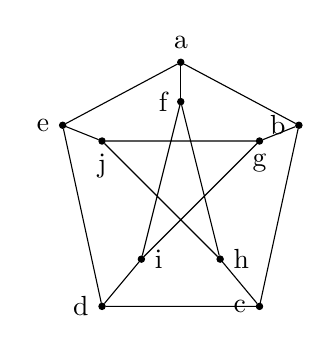
\begin{tikzpicture}
		\node(1) at (-1,1)[circle,fill=black,text=white,inner sep=.8pt,label=below:j,draw]{};
		\node(2) at (1,1)[circle,fill=black,text=white,inner sep=.8pt,label=below:g,draw]{};
		\node(3) at (-.5,-.5)[circle,fill=black,text=white,inner sep=.8pt,label=right:i,draw]{};
		\node(4) at (.5,-.5)[circle,fill=black,text=white,inner sep=.8pt,label=right:h,draw]{};
		\node(5) at (0,1.5)[circle,fill=black,text=white,inner sep=.8pt,label=left:f,draw]{};
		\node(6) at (-1.5,1.2)[circle,fill=black,text=white,inner sep=.8pt,label=left:e,draw]{};
		\node(7) at (0,2)[circle,fill=black,text=white,inner sep=.8pt,label=above:a,draw]{};
		\node(8) at (1.5,1.2)[circle,fill=black,text=white,inner sep=.8pt,label=left:b,draw]{};
		\node(9) at (-1,-1.1)[circle,fill=black,text=white,inner sep=.8pt,label=left:d,draw]{};
		\node(10) at (1,-1.1)[circle,fill=black,text=white,inner sep=.8pt,label=left:c,draw]{};
		
		\draw (1) to (2) to (3) to (5) to (4) to (1) to (6)  to (7) to (8) to (10) to (9) to (3);
		\draw(9) to (6);
		\draw(5) to (7);
		\draw(4) to (10);
		\draw(8) to (2);
		
	\end{tikzpicture}
	
\end{document}